\documentclass[10pt,journal]{./IEEE_latex_class/IEEEtran}

% In order to reference go to http://truben.no/latex/bibtex/

% *** CITATION PACKAGES ***
\usepackage{cite}

% *** GRAPHICS RELATED PACKAGES ***
%
\ifCLASSINFOpdf
   \usepackage[pdftex]{graphicx}
  % declare the path(s) where your graphic files are
  \graphicspath{{./Figures/}}
  % and their extensions so you won't have to specify these with
  % every instance of \includegraphics
  \DeclareGraphicsExtensions{.pdf,.jpeg,.png}
\else
  % or other class option (dvipsone, dvipdf, if not using dvips). graphicx
  % will default to the driver specified in the system graphics.cfg if no
  % driver is specified.
  % \usepackage[dvips]{graphicx} 
  % declare the path(s) where your graphic files are 
  % \graphicspath{{../eps/}}   
  % and their extensions so you won't have to specify these with
  % every instance of \includegraphics
  % \DeclareGraphicsExtensions{.eps}
\fi


% *** MATH PACKAGES ***
\usepackage[cmex10]{amsmath}
\usepackage{amssymb}

% correct bad hyphenation here
\hyphenation{op-tical net-works semi-conduc-tor}

%  OTHER PACKAGES

\usepackage{float,amsfonts,multicol,fancyvrb,lastpage,ragged2e,url,color,lipsum,enumerate,todonotes}

\usepackage[caption=false]{subfig}



\begin{document}

%
% paper title
% can use linebreaks \\ within to get better formatting as desired
\title{Computational design of RNA-based oscillatory circuits}

\author{J.~Binysh
        \\ \IEEEmembership{* University of Warwick, Complexity Department}
        \vspace{-3em}}

% The paper headers
\markboth{hi}%
{Optimisation of Car Electronics}

% make the title area
\maketitle

% This defines the title + page out of # of pages at the heading of the pages
\thispagestyle{empty}

\newcommand{\MYheader}{\smash{\scriptsize

\hfil\parbox[t][\height][t]{\textwidth}{\centering {\normalsize
Place conference title here}}\hfil\hbox{}}}
\makeatletter

\if@twoside
  \def\ps@headings{%
      \let\@oddfoot\@empty\let\@evenfoot\@empty
      \def\@evenhead{\small\thepage\hfil\leftmark\strut\vadjust{\vskip .1ex\hrule}}%
      \def\@oddhead{\small\rightmark\hfil\thepage\strut\vadjust{\vskip .1ex\hrule}}%
      \let\@mkboth\markboth
    \def\chaptermark##1{%
      \markboth{\scshape%
        \ifnum \c@secnumdepth >\m@ne
            \@chapapp\ \thechapter. \ %
        \fi
        ##1}{}}%
    \def\sectionmark##1{%
      \markright{\scshape%
        \ifnum \c@secnumdepth >\z@
          \thesection. \ %
        \fi
        ##1}}}
\else
  \def\ps@headings{%
    \let\@oddfoot\@empty
    \def\@oddhead{{\slshape\rightmark}\hfil\thepage\ of\ \pageref{LastPage} \strut\vadjust{\vskip .1ex\hrule}}%
    \let\@mkboth\markboth
    \def\chaptermark##1{%
      \markright{\scshape%
        \ifnum \c@secnumdepth >\m@ne
            \@chapapp\ \thechapter. \ %
        \fi
        ##1}}}
\fi
\makeatother

\makeatother

% make changes take effect
\pagestyle{headings}
% adjust as needed
%\addtolength{\footskip}{0\baselineskip}
%\addtolength{\textheight}{-0.1\baselineskip}

\begin{abstract}
the abstract
\end{abstract}



\IEEEpeerreviewmaketitle


\section{Introduction}
\label{sec: Intro}
The process of gene expression can be briefly summarised as follows: DNA is read, and a copy of it is made, in the form of an RNA molecule (this is called \textit{transcription}). This RNA molecule (known as messenger RNA, or mRNA) makes its way to a piece of cellular machinery called the Ribosome, which reads it, and makes a protein - which protein is made depends on the DNA sequence originally read (\textit{translation}).  

 The path from genetic transcription to protein expression is naturally regulated in many ways \cite{MolecularBiology}. This regulation allows the cell to control protein expression, and so cell behaviour, in response to various environmental cues. The natural cell machinery in place to perform this regulation offers rich possibilities for modification, and an important goal within synthetic biology is to understand and manipulate it.

As well as acting as the intermediate between DNA and protein, RNA molecules play direct and important roles in regulating cell behaviour \cite{Isaacs2006}. For the synthetic biologist looking to engineer regulation of genetic circuitry, RNA's offers an attractive alternative to more traditional methods, which typically involve using proteins to regulate DNA transcription. In comparison to proteins, it is relatively straightforward to predict the structure and function of an RNA from its sequence using physiochemical models. Recently, this has been exploited to computationally design DNA sequences encoding synthetic sRNA's, with regulatory behaviour that can be predicted \cite{Rodrigo2013}\cite{Rodrigo2012}.

This report will focus on one such system, introduced in \cite{Rodrigo2012}. It will extend existing understanding of the system beyond the qualitative, by proposing a quantitative model of gene expression, in the form of a set of ODE's, and fitting it to available time series data to estimate the model's unknown parameters.

The report is structured as follows. In section \ref{The sRNA regulatory system} we review the sRNA regulatory system we will consider. In section \ref{Results and Discussion} 
we propose a set of ODE's to model the system, and estimate its unknown parameters by fitting to time series data. Finally, in section \ref{Conclusions and Further work}, we conclude, and suggest directions for further work.

 \begin{itemize}
 \item goal of the project - emph on quantitative modelling of biological system and data, getting a quantitative model, finding its parameters.
 \item Biological background, taken from those 3 papers.
 \item give structure of the report.
 \end{itemize}

\section{The sRNA regulatory system}
\label{The sRNA regulatory system}

 \begin{itemize}
 \item  
 \item

 \end{itemize}
 
 

\begin{figure}[H]
\centering
\includegraphics[trim = 60 630 300 30,page=2,clip = true]{pnas1203831109.pdf}
\caption{A network with an intuitively clear community structure, which is captured by the partition chosen, shown in gray. Image reproduced from \cite{community_figure}}
\label{community}
\end{figure}



%%%
%NEW SECTION%
%%%
\section{Results and Discussion}
\label{Results and Discussion}


%NEW SUBSECTION%

\subsection{Model Derivation}

 \begin{itemize}
 \item introduce the proposed ode model, explain its biology.
 \item Biological background, taken from those 3 papers.
 \end{itemize}

%NEW SUBSECTION%

\subsection{Parameter Estimation}
 \begin{itemize}
\item basically the whole project.
\cite{Isaacs2006}
 \end{itemize}
 
\section{Conclusions and Further work}
\label{Conclusions and Further work}


% references section
\bibliographystyle{./IEEE_bibtex_class/IEEEtran}
\bibliography{./IEEE_bibtex_class/IEEEabrv,library}


\end{document}